% $Id: board2a.tex 9493 2021-10-26 22:07:41Z mskala $

%
% MSK 010 Board 2, variant A build instructions
% Copyright (C) 2017, 2018, 2021  Matthew Skala
%
% This program is free software: you can redistribute it and/or modify
% it under the terms of the GNU General Public License as published by
% the Free Software Foundation, version 3.
%
% This program is distributed in the hope that it will be useful,
% but WITHOUT ANY WARRANTY; without even the implied warranty of
% MERCHANTABILITY or FITNESS FOR A PARTICULAR PURPOSE.  See the
% GNU General Public License for more details.
%
% You should have received a copy of the GNU General Public License
% along with this program.  If not, see <http://www.gnu.org/licenses/>.
%
% Matthew Skala
% https://northcoastsynthesis.com/
% mskala@northcoastsynthesis.com
%

\chapter{Building Board 2 (Variant A)}

The recommended order for building this module is to assemble Board 2, the
one further from the front panel, first.  That will make it easier to get
all the physical positioning right for the components that bridge between
the boards or pass through the panel.  But before you start assembling Board
2, you must decide which variant you want to build.  Each one has a
different selection of eight nominal output frequencies.  Follow the
instructions in \emph{one} of the three ``Building Board 2'' chapters, depending on
which variant you want, before proceeding to the chapter called ``Building
Board 1.''  It's a choose your own module adventure!

\emph{This chapter contains the build instructions for Variant A, which has
the following nominal output frequencies and periods:}

\begin{tabular}{cc}
frequency & period \\ \hline
16mHz & 63s \\
60mHz & 16s \\
190mHz & 5.3s \\
410mHz & 2.4s \\
720mHz & 1.4s \\
1.3Hz & 750ms \\
4.8Hz & 210ms \\
16Hz & 63ms
\end{tabular}

If you have chosen Variant~A, use a permanent marker or some enamel paint to
fill in the ``A'' circle at the lower right of the front panel, so that you
can easily keep track of which module the one you're building now is, in a
system that might someday contain several MSK~010 modules.

Note that I'm describing a separate step for each component value,
and I built one that way in order to take a photo at each step, but if you
are reasonably confident about your skills you may find it easier to
populate all or most of the board (i.e.\ put the components in place) and
then solder them all at once.  Except where noted, the order in which you
add components does not matter much; but do note that you should solder the
board-to-board connector before the larger capacitors, because otherwise
they block access to it.

\section{Preliminaries}

Count out the right number of everything according to the bill of materials. 
There is an abbreviated BOM for Board~2, and a few items from Board~1 used
during the assembly of Board~2, in Table~\ref{tab:b2bom}.

\begin{table*}
{\centering
\fbox{This table is not a substitute for the text instructions.}
\vspace{\baselineskip}

\begin{tabular}{rp{1in}cp{3in}}
  \textbf{Qty} & \textbf{Ref} & \textbf{Value/Part No.} & \\ \hline
\input{bomdata-2a.tex}
\end{tabular}\par}
\caption{Bill of Materials for assembling Board~2.}\label{tab:b2bom}
\end{table*}

\section{Decoupling capacitors}

The four axial ceramic 0.1$\mu$F decoupling capacitors, C9, C10, C19, and
C20, are shown on the board by a special symbol without their reference
designators.

\noindent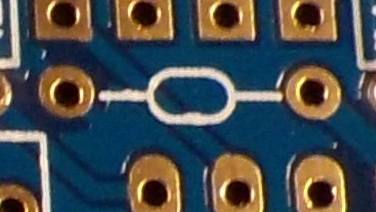
\includegraphics[width=\linewidth]{decoup-symbol.jpg}

Install these four capacitors where the symbol appears.  They are not
polarized and may be installed in either orientation.  These capacitors act
as filters for the power supplies to the op amp chips, reducing any coupling
of high-frequency noise between them and the rest of the synthesizer.

\noindent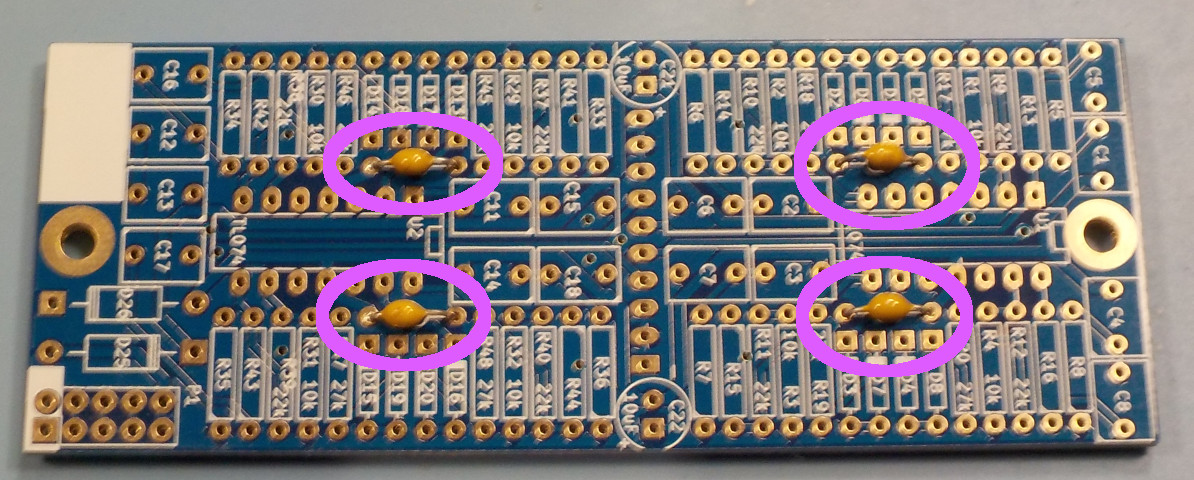
\includegraphics[width=\linewidth]{cap-decoup.jpg}

\section{Fixed resistors}

Resistors are never polarized.  I like to install mine in a consistent
direction for cosmetic reasons, but this is electrically unnecessary.  In
this module, metal film 1\%\ resistors are recommended for all fixed-value
resistors.  These will usually have blue bodies and four colour bands
designating the value, plus a fifth band (always brown\footnote{It also
happens, because of the way we choose resistor values, that the third band
will be black for all the resistors used in this module and nearly all the
resistors used in North Coast modules in general.}) for the tolerance,
and these are the types of resistors shipped in the North Coast kits.
Accordingly, I mention only the four value band colours for this type of
resistor; if you are using resistors with other codes, you are responsible
for knowing them.  Note that colour codes on metal film 1\% resistors are
often ambiguous (reading from one end or the other end may give two
different values, both plausible) and some of the colours are hard to
distinguish anyway.  If in doubt, always measure with an ohmmeter before
soldering the resistor in place.

The physical size of the resistors may vary, and details like the exact
colour of the bluish background.  You can see some of that variation in the
photos in these instructions.  Some of the resistance values used in this
module are hard to find, and we source different values from different
suppliers, so not all the resistors in a kit will necessarily be from the
same manufacturer, nor match on non-critical specifications like power
rating and physical size.

Install the eight 10k$\Omega$ (brown-black-black-red) resistors R1 to R4 and
R29 to R32.  These form part of the gain-control network for the amplifiers,
acting as a reference for the other components to balance against.  Do
not confuse these with similar-looking resistors for other power-of-ten
values, such as 1k$\Omega$ or 1M$\Omega$; those have the same colour code
except with the red replaced by other colours.

Be aware that one leg of each of these resistors is connected to the ground
plane of the circuit board, a fact evident from the cross-shaped pattern of
``thermal relief'' connections around the solder pad.  These joints, and
other grounded pins throughout the module, may require extra time and heat
to solder because each one is connected to large chunks of copper on both
sides of the board that tend to conduct heat away from the joint.  The
thermal relief design is supposed to reduce this effect, but in practice,
especially when using a low-wattage iron, it only helps to a limited degree.

\noindent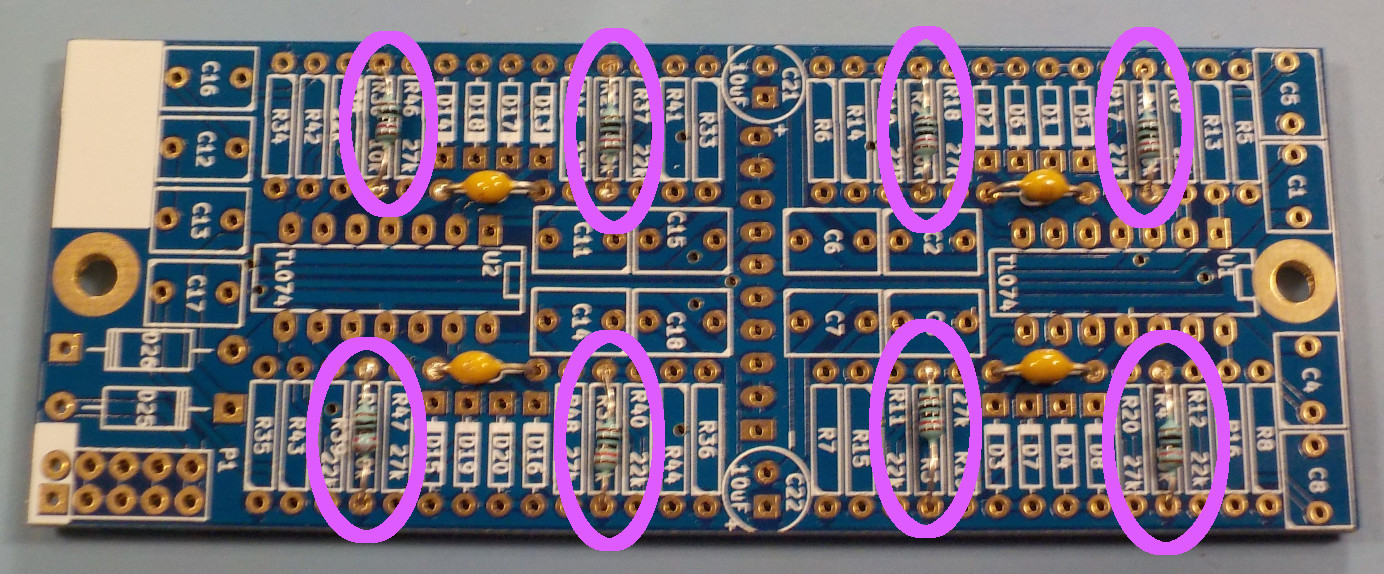
\includegraphics[width=\linewidth]{res-10k.jpg}

Install the eight 22k$\Omega$ (red-red-black-red) resistors R9 to R12 and
R37 to R40.  These set the small-signal gain for the amplifiers by balancing
against the 10k$\Omega$ resistors.  Do not confuse these with the very
similar-looking 27k$\Omega$ resistors, which have the second band violet
instead of red.  Swapping the two values will result in bad output levels,
most likely too high with clipping, possibly too low.

\noindent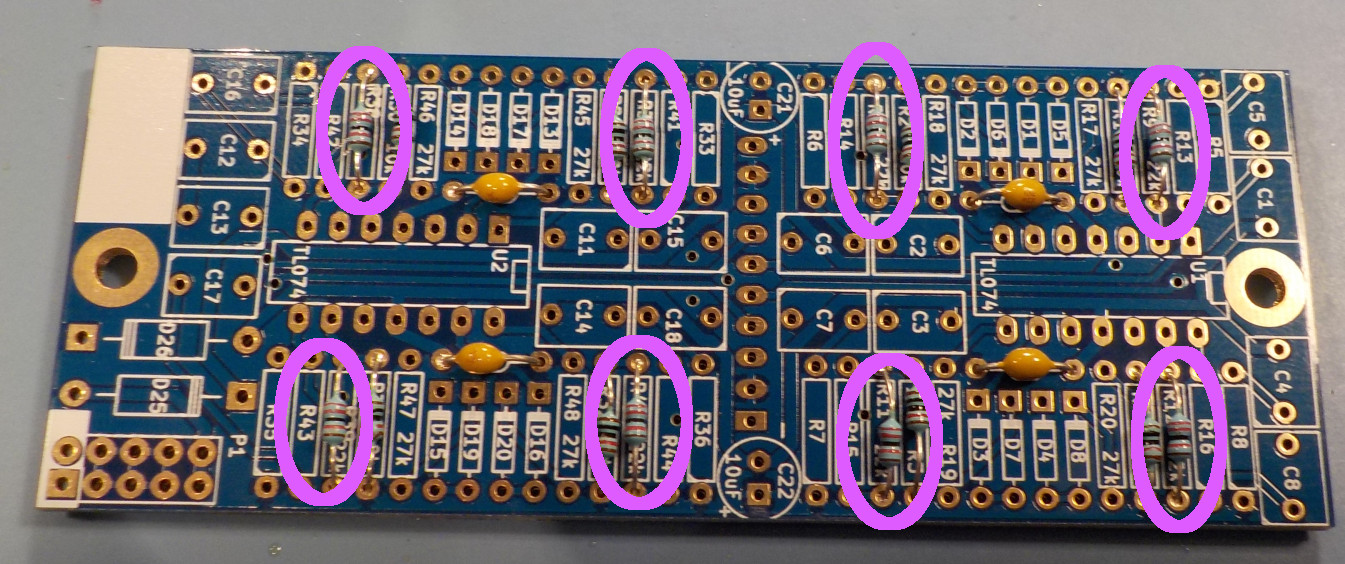
\includegraphics[width=\linewidth]{res-22k.jpg}

Install the eight 27k$\Omega$ (red-violet-black-red) resistors R17 to R20
and R45 to R48.  These are coupled into the circuit under control of the
Zener diodes to reduce the gain as needed for the desired output levels.

\noindent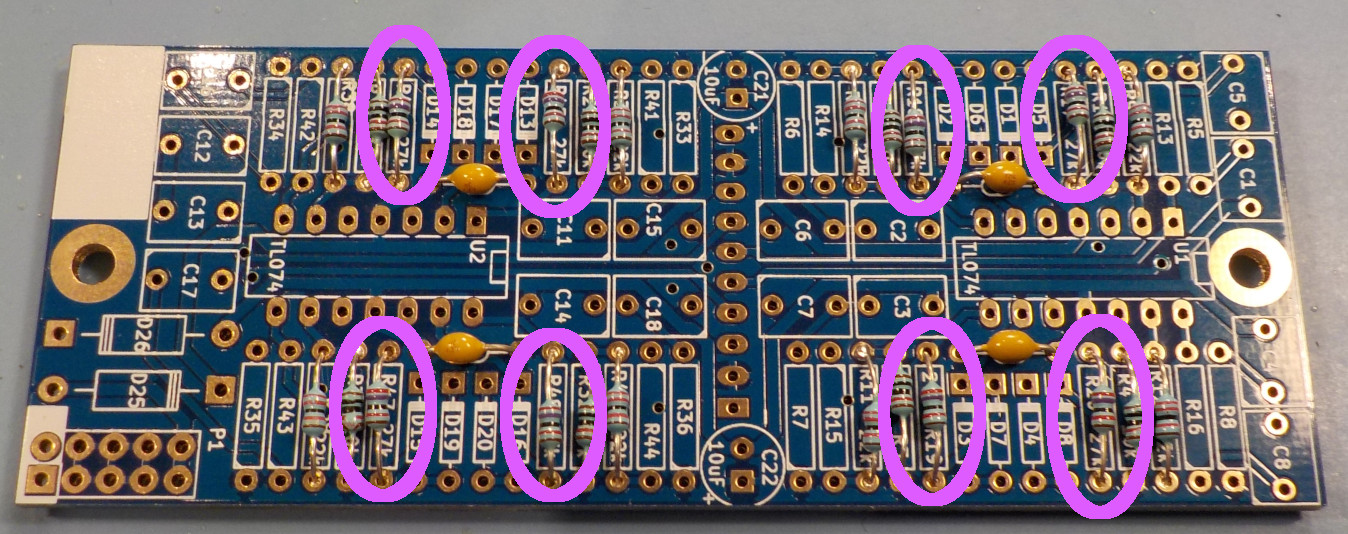
\includegraphics[width=\linewidth]{res-27k.jpg}

The next eight resistor values (two of each) are installed in locations on
the board marked with reference designators (like ``R5'') but no values. 
That is because these are meant to be installed in different locations
depending on which variant of the module you are building.  The
correspondence between locations and values for Variant~A is shown in
Figure~\ref{fig:board-stuffing-2a}.  Follow the diagram and these
instructions carefully, because it is easy to make a mistake.

All these resistors are used to determine the frequencies of the
oscillators, two for each oscillator.  Installing the wrong timing resistor
value in one of the oscillators, but the same wrong value for both of the
two timing resistors, will result in oscillation at the wrong frequency. 
Installing two different resistor values in one oscillator will probably
result in its failure to oscillate at all.

\def\RVA{100k$\Omega$}\def\CVA{0.10$\mu$F}\def\TVA{63ms}\def\FVA{16Hz}
\def\RVB{150k$\Omega$}\def\CVB{0.22$\mu$F}\def\TVB{210ms}\def\FVB{4.8Hz}
\def\RVC{1.2M$\Omega$}\def\CVC{0.10$\mu$F}\def\TVC{750ms}\def\FVC{1.3Hz}
\def\RVD{1.0M$\Omega$}\def\CVD{0.22$\mu$F}\def\TVD{1.4s}\def\FVD{720mHz}
\def\RVE{390k$\Omega$}\def\CVE{1.0$\mu$F}\def\TVE{2.4s}\def\FVE{410mHz}
\def\RVF{1.8M$\Omega$}\def\CVF{0.47$\mu$F}\def\TVF{5.3s}\def\FVF{190mHz}
\def\RVG{5.6M$\Omega$}\def\CVG{0.47$\mu$F}\def\TVG{16s}\def\FVG{60mHz}
\def\RVH{10M$\Omega$}\def\CVH{1.0$\mu$F}\def\TVH{63s}\def\FVH{16mHz}

\begin{figure*}
\centering\begin{tikzpicture}
  \node at (0,0) {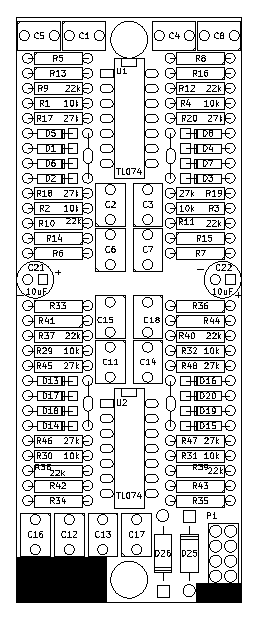
\includegraphics{rc2.eps}};
  \node[rectangle,draw,dashed,blue,very thick,inner sep=0.6cm]
    (o1) at (-1.15,4.4) {~~~~~~};
  \node[rectangle,draw,dashed,blue,very thick,inner sep=0.8cm]
    (o2) at (-1.0,1.4) {~~~~};
  \node[rectangle,draw,dashed,blue,very thick,inner sep=0.8cm]
    (o3) at (-1.0,-0.5) {~~~~};
  \node[rectangle,draw,dashed,blue,very thick,inner sep=0.65cm]
    (o4) at (-1.35,-3.53) {};
  \node[rectangle,draw,dashed,blue,very thick,inner sep=0.6cm]
    (o5) at (1.15,4.4) {~~~~~~};
  \node[rectangle,draw,dashed,blue,very thick,inner sep=0.8cm]
    (o6) at (1.0,1.4) {~~~~};
  \node[rectangle,draw,dashed,blue,very thick,inner sep=0.8cm]
    (o7) at (1.0,-0.5) {~~~~};
  \node[rectangle,draw,dashed,blue,very thick,inner sep=0.65cm]
    (o8) at (0.66,-3.53) {~~~~~~~~~~~~};
  \node at (-4.5,5.0) {\small\begin{tabular}{rl}
    \multicolumn{2}{c}{J5} \\
    C1, C5 & \CVA \\
    R5, R13 & \RVA \\
    $t$ & \TVA \\
    $f$ & \FVA
  \end{tabular}} edge[very thick,blue] (o1);
  \node at (-4.5,-0.7) {\small\begin{tabular}{rl}
    \multicolumn{2}{c}{J6} \\
    C11, C15 & \CVB \\
    R33, R41 & \RVB \\
    $t$ & \TVB \\
    $f$ & \FVB
  \end{tabular}} edge[very thick,blue] (o3);
  \node at (-4.5,1.8) {\small\begin{tabular}{rl}
    \multicolumn{2}{c}{J7} \\
    C2, C6 & \CVC \\
    R6, R14 & \RVC \\
    $t$ & \TVC \\
    $f$ & \FVC
  \end{tabular}} edge[very thick,blue] (o2);
  \node at (-4.5,-4.0) {\small\begin{tabular}{rl}
    \multicolumn{2}{c}{J8} \\
    C12, C16 & \CVD \\
    R34, R42 & \RVD \\
    $t$ & \TVD \\
    $f$ & \FVD
  \end{tabular}} edge[very thick,blue] (o4);
  \node at (4.5,-0.7) {\small\begin{tabular}{rl}
    \multicolumn{2}{c}{J1} \\
    C14, C18 & \CVE \\
    R36, R44 & \RVE \\
    $t$ & \TVE \\
    $f$ & \FVE
  \end{tabular}} edge[very thick,blue] (o7);
  \node at (4.5,1.8) {\small\begin{tabular}{rl}
    \multicolumn{2}{c}{J2} \\
    C3, C7 & \CVF \\
    R7, R15 & \RVF \\
    $t$ & \TVF \\
    $f$ & \FVF
  \end{tabular}} edge[very thick,blue] (o6);
  \node at (4.5,-4.0) {\small\begin{tabular}{rl}
    \multicolumn{2}{c}{J3} \\
    C13, C17 & \CVG \\
    R35, R43 & \RVG \\
    $t$ & \TVG \\
    $f$ & \FVG
  \end{tabular}} edge[very thick,blue] (o8);
  \node at (4.5,5.0) {\small\begin{tabular}{rl}
    \multicolumn{2}{c}{J4} \\
    C4, C8 & \CVH \\
    R8, R16 & \RVH \\
    $t$ & \TVH \\
    $f$ & \FVH
  \end{tabular}} edge[very thick,blue] (o5);
\end{tikzpicture}\par
\caption{Populating Board~2 for Variant~A}\label{fig:board-stuffing-2a}
\end{figure*}

Install the two 100k$\Omega$ (brown-black-black-orange) resistors R5
and R13.  Do not confuse these with other power-of-ten values.

\noindent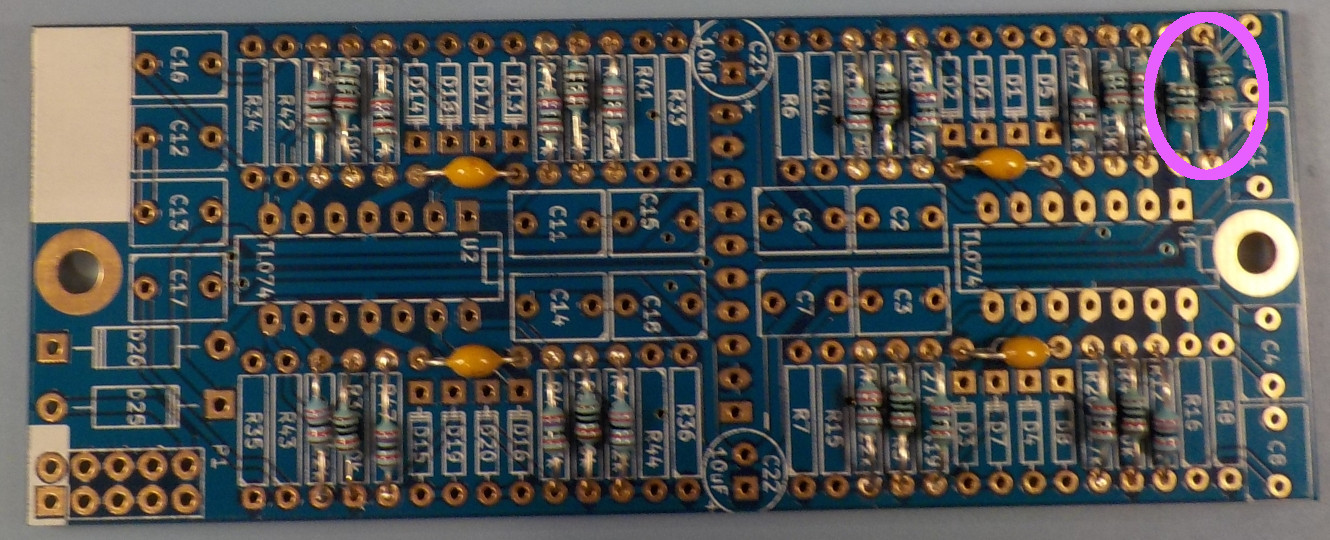
\includegraphics[width=\linewidth]{res-100kA.jpg}

Install the two 150k$\Omega$ (brown-green-black-orange) resistors R33
and R41.

\noindent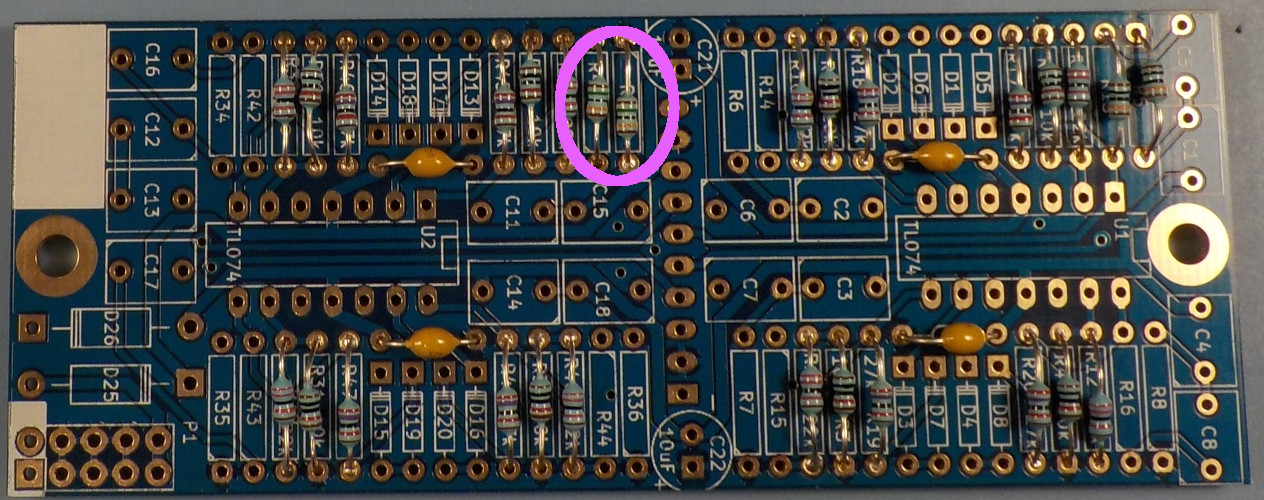
\includegraphics[width=\linewidth]{res-150kA.jpg}

Install the two 390k$\Omega$ (orange-white-black-orange) resistors R36
and R44.

\noindent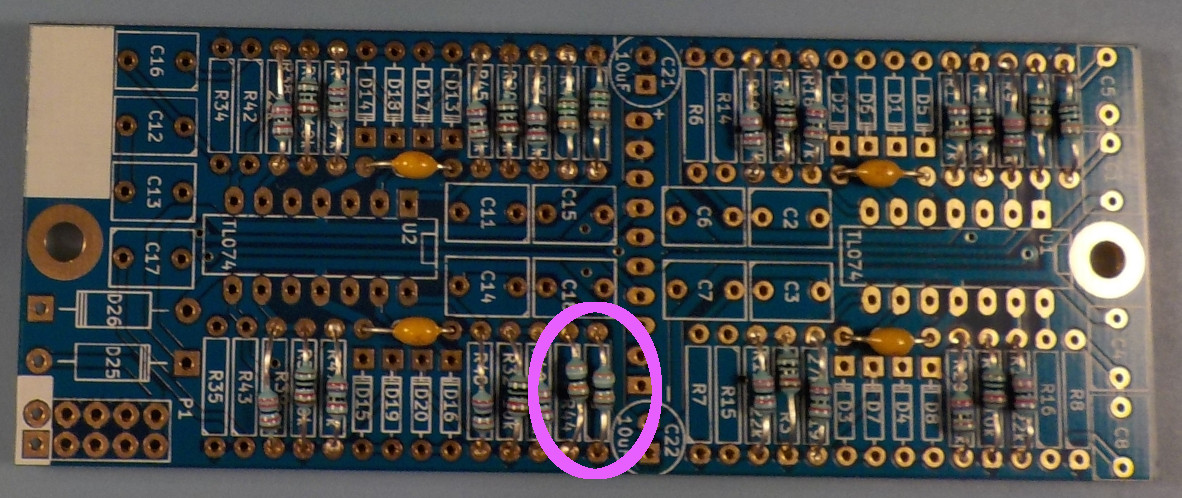
\includegraphics[width=\linewidth]{res-390kA.jpg}

Install the two 1.0M$\Omega$ (brown-black-black-yellow) resistors R34
and R42.  Do not confuse these with other power-of-ten values.

\noindent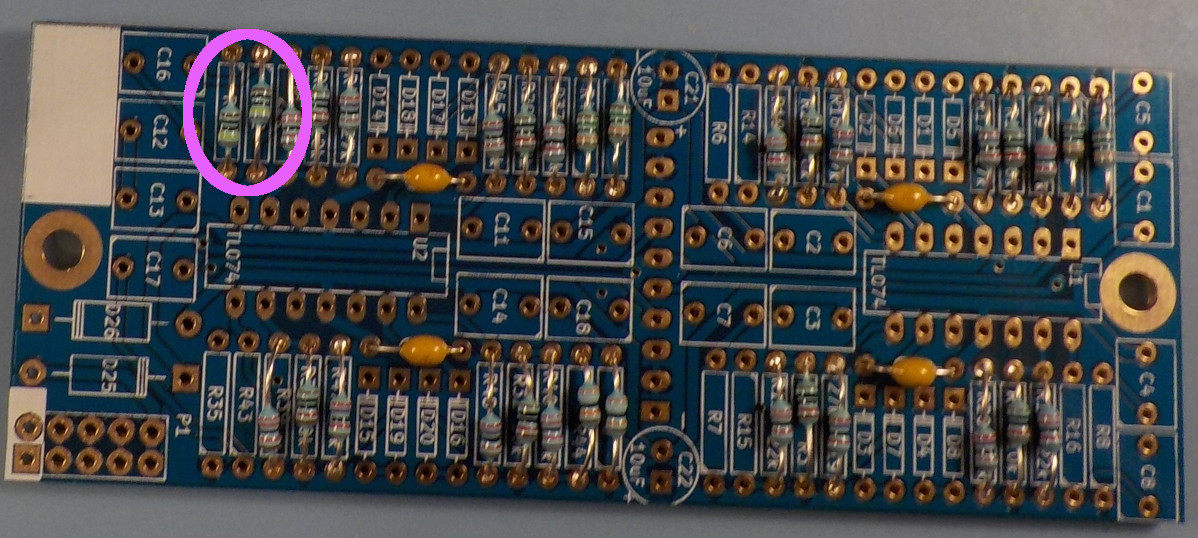
\includegraphics[width=\linewidth]{res-1MA.jpg}

Install the two 1.2M$\Omega$ (brown-red-black-yellow) resistors R6 and
R14.

\noindent\includegraphics[width=\linewidth]{{res-1.2MA}.jpg}

Install the two 1.8M$\Omega$ (brown-gray-black-yellow) resistors R7
and R15.

\noindent\includegraphics[width=\linewidth]{{res-1.8MA}.jpg}

Install the two 5.6M$\Omega$ (green-blue-black-yellow) resistors R35
and R43.

\noindent\includegraphics[width=\linewidth]{{res-5.6MA}.jpg}

Install the two 10M$\Omega$ (brown-black-black-green) resistors R8 and
R16.  Do not confuse these with other power-of-ten values.

\noindent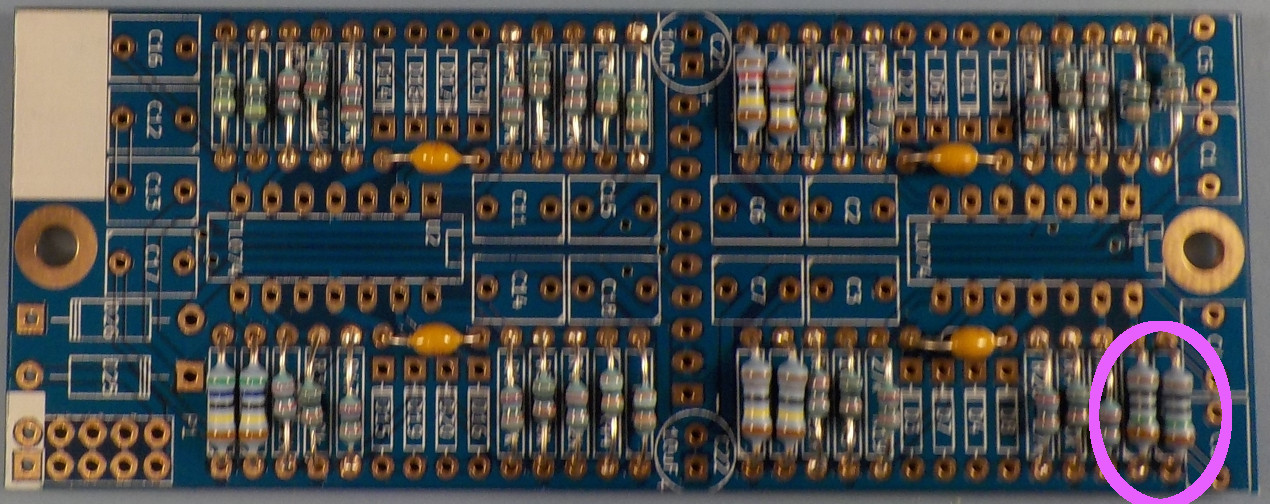
\includegraphics[width=\linewidth]{res-10MA.jpg}

\section{Board to board connectors}

It is important to solder the male header connector that links Board~2 to
Board~1 at this time, before adding the film and electrolytic capacitors,
because the capacitors surround the solder pads on the front of Board~2 in a
way that makes it difficult to work on the connector without damaging the
capacitors.  For best alignment, you should solder the male connector while
it is mated with the female connector on Board~1, and it's convenient to
solder the Board~1 connector at this time too.

Assemble the two boards and the two connectors using the M3 machine screws,
and 10mm and 11mm standoffs, as shown.  The 11mm standoffs should separate
the two boards; I suggest using the 10mm standoffs instead of hex nuts for
this temporary assembly because they're easier to tighten by hand.  Do not
confuse the two lengths.  Solder the connectors on both boards.  Then
disassemble them, and set aside the hardware and Board~1 for later.

\noindent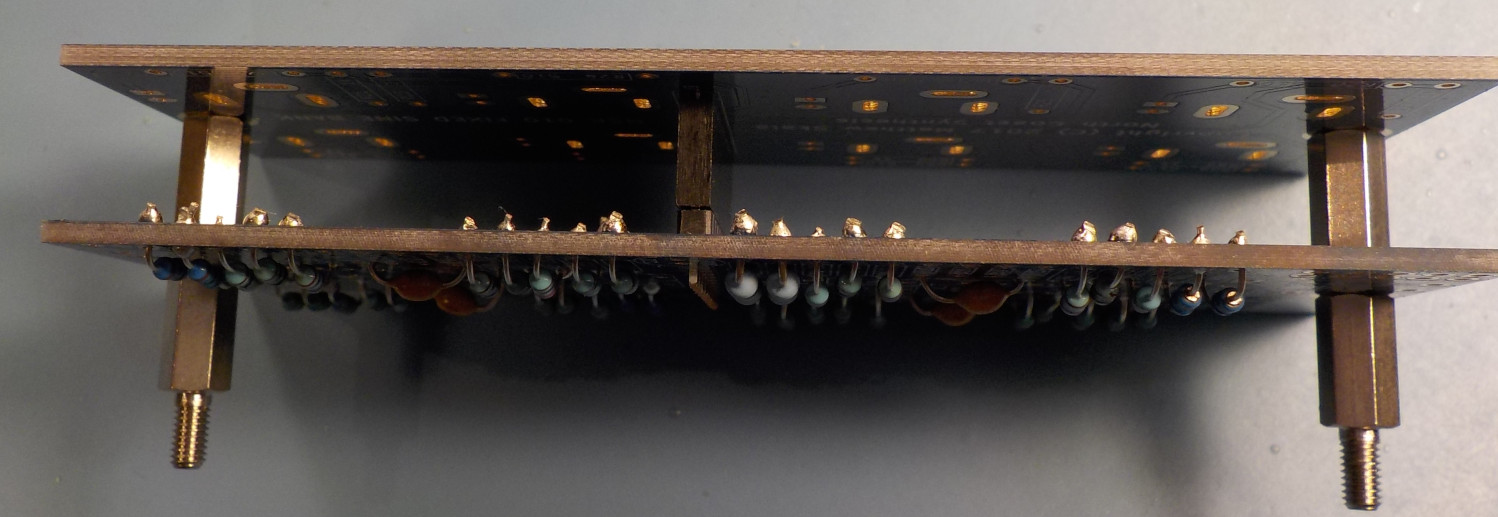
\includegraphics[width=\linewidth]{b2b-stack.jpg}

\section{Semiconductors}

Install the sixteen 1N5229B 4.3V Zener diodes D1 to D8 and D13 to D20. 
These control the output level of the oscillators, by gradually bringing the
27k$\Omega$ resistors into the circuit as the level increases to back down
the gain until it reaches equilibrium.  They are polarized components and it
is important to install them right way round.  Each diode is packaged inside
a pink glass bead with a black stripe at one end; that end is the
\emph{cathode}.  The silkscreen markings on the board have a corresponding
stripe and the diodes should be installed with their stripes matching the
markings on the board.  The solder pads for the cathodes are also square
instead of round; and the diodes are arranged so that all the cathodes point
inward from the edge of the board.  Installing one of these diodes backwards
will probably result in the output level of the corresponding oscillator
being much too low, as well as some asymmetric (second harmonic) distortion
in the waveform.

\noindent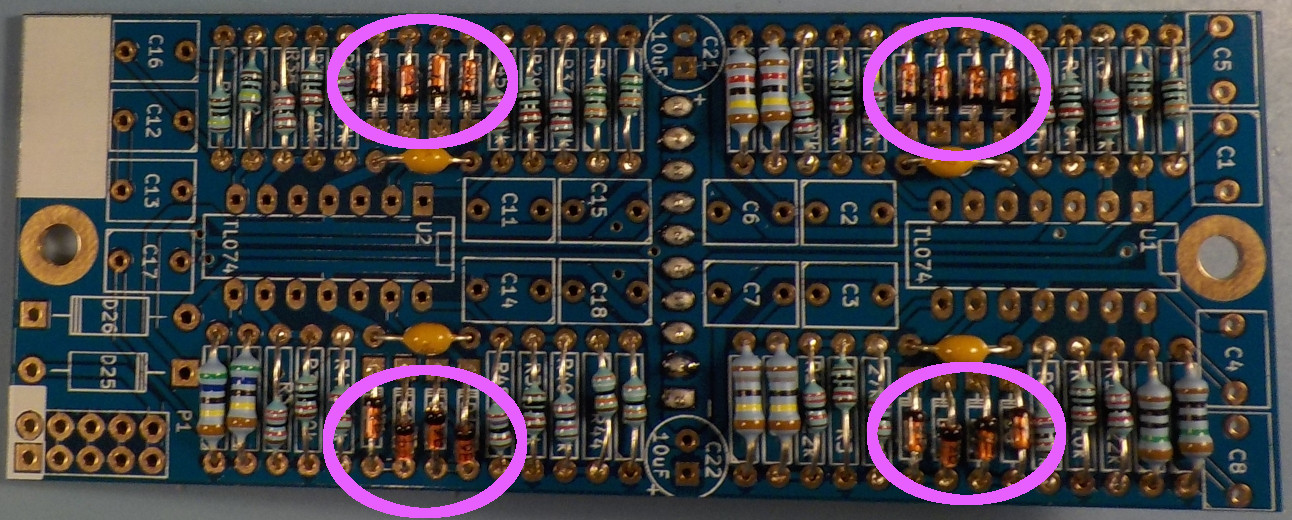
\includegraphics[width=\linewidth]{zenerA.jpg}

The 1N5229B diodes are the only small glass diodes in an MSK~010 kit, but be
warned that if you're doing other electronic construction, then you will
probably have many other small glass diodes on hand (for instance, the very
popular 1N4148 general-purpose type) and they all look pretty much
identical, distinguished only by their electrical properties and
near-microscopic code numbers etched onto the glass.  Be careful not to mix
these diodes up with other types of diodes.  Substituting general-purpose
switching diodes in this circuit will probably give you output levels that
are much too high.

Install the two 1N5818 or SBA130 Schottky rectifier diodes D25 and D26. 
These are for reverse-voltage protection; they cut off power to the module
when the power plug is backwards.  They are polarized and it is important to
install them in the right direction.  As with the Zeners, these diodes will
be marked with stripes indicating their cathodes (here, probably white or
light grey paint on a black or dark grey plastic package) and those stripes
should match the stripes on the PCB silkscreen.  The cathode solder pads are
also square.  Installing these backwards means they will have the opposite
of the intended protective effect.

\noindent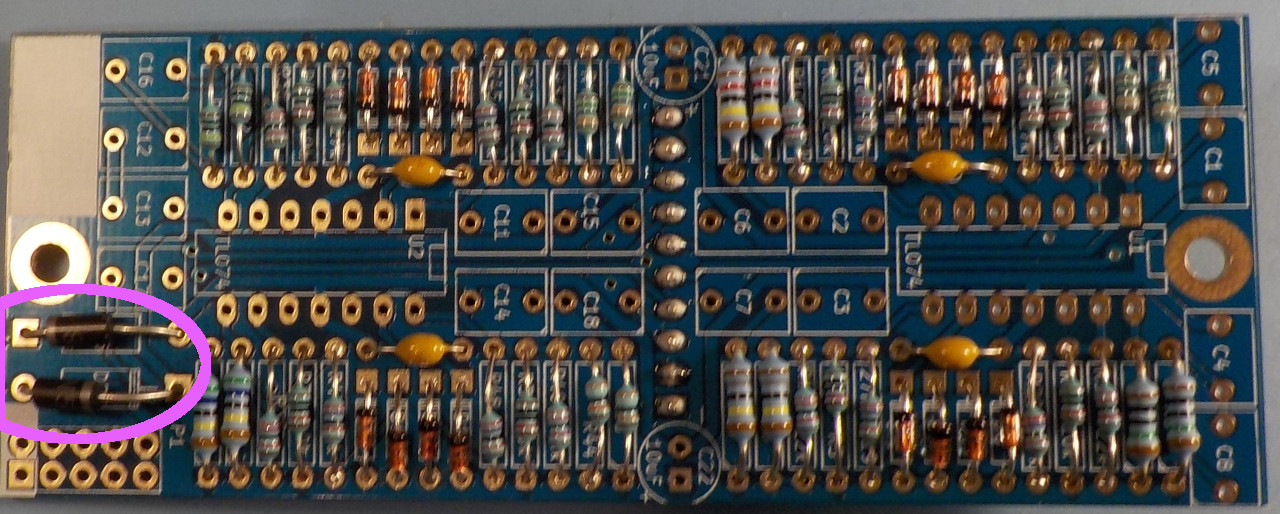
\includegraphics[width=\linewidth]{schottkyA.jpg}

Install the two 14-pin DIP sockets for the TL074 quad op amp chips, U1 and
U2.  These chips provide amplification to keep the oscillators running.  The
sockets themselves do not care which direction you install them, but it is
critically important that the chips installed in the sockets should be
installed in the right direction.  To help with that, the sockets will
probably be marked with notches at one end (indicating the end where Pin~1
and Pin~14 are located) and you should install the sockets so that the
notched ends match the notches shown on the PCB silkscreen.  The solder pad
for Pin~1 is also distinguished by being rectangular instead of rounded.

Installing DIP sockets without having them tilted at a funny angle can be
tricky.  I recommend inserting the socket in the board, taping it in place
on the component side with vinyl electrical tape, then soldering one pin on
one corner and checking that the socket is snug against the board before
soldering the other pins.  That way, if you accidentally solder the first
pin with the socket tilted, it will be easier to correct (only one pin to
desolder instead of all of them).

\noindent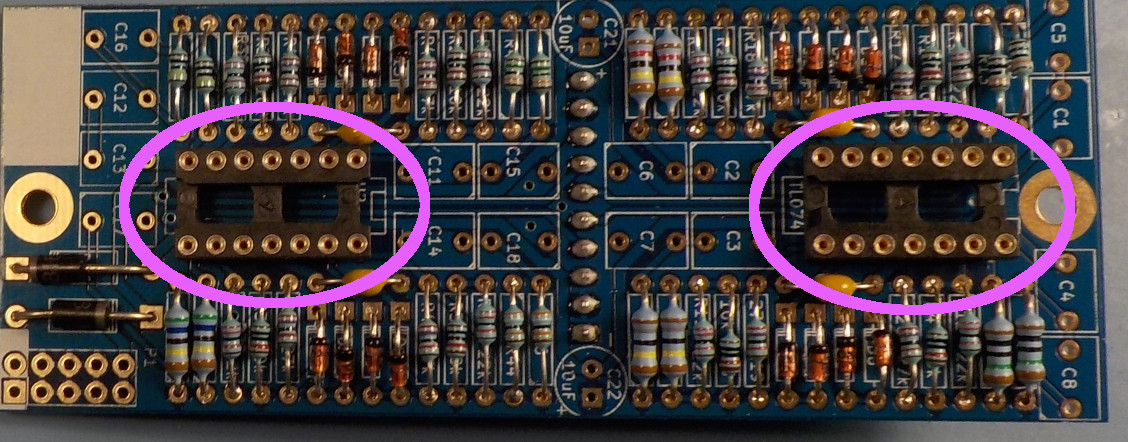
\includegraphics[width=\linewidth]{dip-2A.jpg}

If you somehow manage to solder an entire socket in backwards, don't try to
desolder it to turn it around.  Just leave it as it is and remember that
when you insert the chip, you must insert it so the chip matches the
markings on the \emph{board}, not the turned-around socket.

\section{Film capacitors}

The film capacitors in this module are used to determine oscillator timing. 
As with the timing resistors, they are marked on the PCB with their
references only, no capacitance values, because they are arranged
differently for the different module variants.  See
Figure~\ref{fig:board-stuffing-2a} for information on which capacitors go
where in this variant.

Be careful to identify the values of the capacitors correctly.  They may all
look very similar.  In some cases the physical sizes of the capacitors vary
with their value (for instance, 1.0$\mu$F will probably be bigger than
0.1$\mu$F), but there may also be different values the same physical size. 
Etched markings on the capacitors will probably use the symbol $\mu$ instead
of a decimal point, such as $\mu$1 to designate 0.1$\mu$F, as opposed to
1$\mu$ for 1.0$\mu$F.  Many digital multimeters will have a ``capacitor
test'' feature which you can use to confirm that you've identified the
capacitors correctly.  Installing the wrong capacitors in an oscillator
will give you the wrong frequency (in case of two capacitors that are the
same wrong value) or no oscillation (in case of two capacitors of different
values).

Also be careful about the physical aspects of installing the capacitors.  I
usually stick them in place with vinyl tape before soldering, but it's
difficult to get them to stay in at a nice angle.  If they're tilted over,
that is only really a cosmetic issue; the circuit should work fine as long
as both electrical connections are made.  These capacitors are also
unpolarized, and will work electrically regardless of the direction in which
they are installed.

Install the four 0.1$\mu$F film capacitors C1, C2, C5, and C6.

\noindent\includegraphics[width=\linewidth]{{cap-0.1uA}.jpg}

Install the four 0.22$\mu$F film capacitors C11, C12, C15, and C16.

\noindent\includegraphics[width=\linewidth]{{cap-0.22uA}.jpg}

Install the four 0.47$\mu$F film capacitors C3, C7, C13, and C17.

\noindent\includegraphics[width=\linewidth]{{cap-0.47uA}.jpg}

Install the four 1.0$\mu$F film capacitors C4, C8, C14, and
C18.\footnote{This photo shows the 10$\mu$F capacitors already installed, but
that's really the next step.}

\noindent\includegraphics[width=\linewidth]{{cap-1.0uA}.jpg}

\section{Electrolytic capacitors}

Install the two 10$\mu$F electrolytic capacitors C21 and C22, which filter
the power supply for the module as a whole.  These are polarized components
and they may explode if installed backwards.  Each one will be marked on its
casing with a stripe and minus signs to indicate the negative lead; the
positive lead will probably also be longer.  These clues should be matched
with the markings on the PCB: plus and minus symbols in the silkscreen and a
square solder pad for the positive (long) lead.

\noindent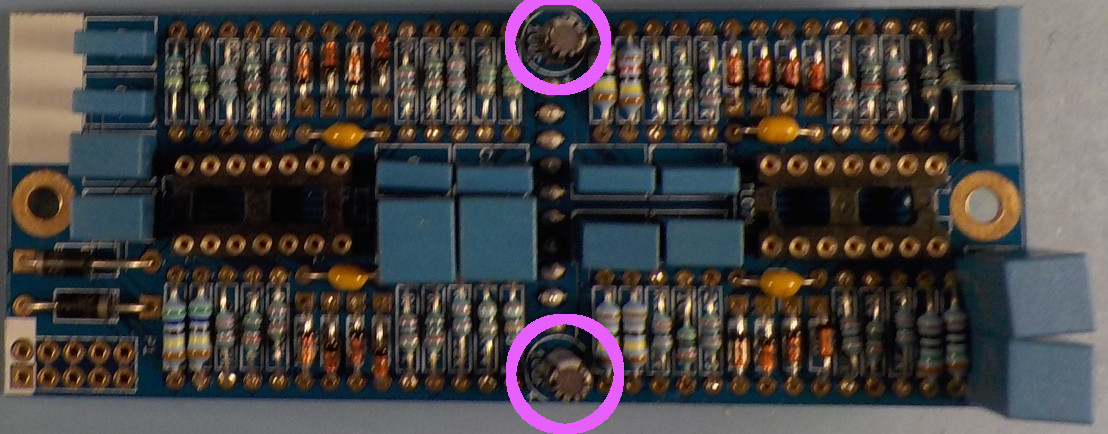
\includegraphics[width=\linewidth]{cap-10uA.jpg}

\section{Eurorack power connector}

Install the 2$\times$5-pin Eurorack power connector.  This connector is not
polarized in itself, although the connection it makes is polarized.  As with
the DIP sockets, you should be careful to get it installed snugly against
the board, not tilted at an angle.  Use vinyl tape or similar to hold it in
place, solder one pin, then check that it is straight before you solder the
other pins.

Be aware that both the connector and the copper connections to it on the PCB
have relatively large thermal mass.  These solder joints will need more
heat than usual; and after you have soldered it, the connector will remain
hot longer than recently-soldered components usually do.  Don't burn
yourself.

The six pins in the centre of the connector, that is all except the four
corner pins, are for grounding and they are all connected together on the
board.  Thus, if you accidentally form solder bridges among these six pins
while installing the connector, don't waste effort trying to remove them;
they will have no electrical effect.

\noindent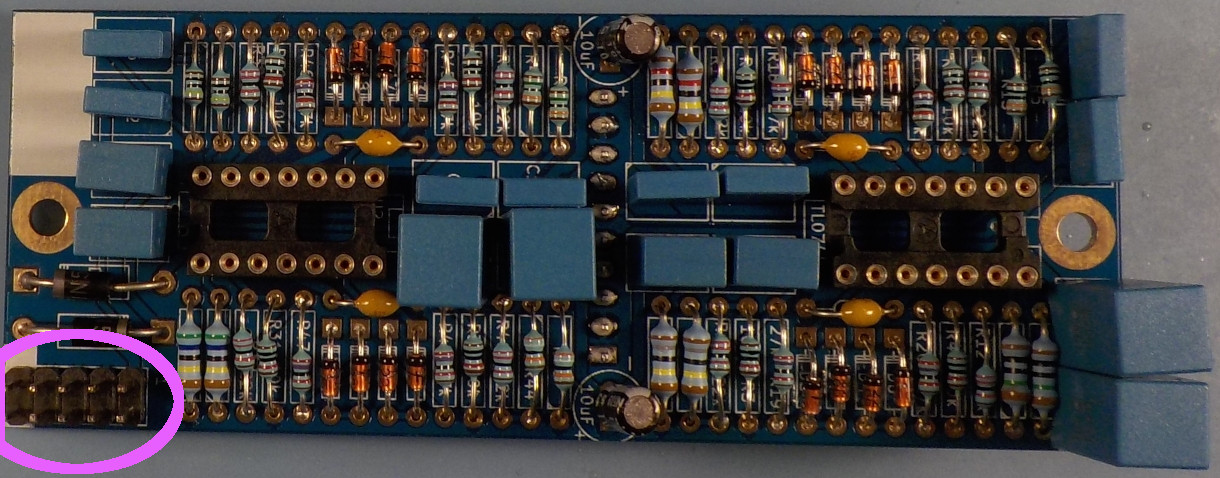
\includegraphics[width=\linewidth]{powerA.jpg}

That's all the components for Board~2.

Because some connections on this board operate at multi-megaohm impedances,
it may be a good idea to clean the flux residue off of Board~2 even if you
are using no-clean flux which would not normally require cleaning.  For
this type of solder flux, or traditional rosin, use isopropyl alcohol for
cleaning.  If you used water-soluble solder flux, then cleaning is
mandatory and you should use water.

In between completed boards is a good time to take a break.
